\section{30 Nov 23 - Activity: Monte Carlo
Integration}\label{nov-23---activity-monte-carlo-integration}

A useful approach to making models of systems is using randomness to
find solutions to problems that are stable or static. One such approach
is called
\href{https://en.wikipedia.org/wiki/Monte_Carlo_integration}{Monte Carlo
integration} that can be used to find particularly problematic
integrals. It's a useful pedagogical introduction to what we are
attempting to do, use
\href{https://en.wikipedia.org/wiki/Monte_Carlo_method}{Monte Carlo
approaches} to model thermodynamical systems using the
\href{https://en.wikipedia.org/wiki/Metropolis\%E2\%80\%93Hastings_algorithm}{Metropolis-Hastings
algorithm}.

\begin{Shaded}
\begin{Highlighting}[]
\ImportTok{import}\NormalTok{ numpy }\ImportTok{as}\NormalTok{ np}
\ImportTok{import}\NormalTok{ matplotlib.pyplot }\ImportTok{as}\NormalTok{ plt}
\ImportTok{import}\NormalTok{ random }\ImportTok{as}\NormalTok{ random}
\OperatorTok{\%}\NormalTok{matplotlib inline}
\end{Highlighting}
\end{Shaded}

\subsection{Finding Pi}\label{finding-pi}

This is a classic use of Monte Carlo integration that illustrates many
of the concepts of the technique. Effectively, we can assume there's a
constant (undetermined) that links that the area of a circle and the
radius squared.

\[A_{circle} = c r^2\]

We assume it's radius squared as a test because we know that boxes go
like length times width and a sqaure with side length \(r\) has:

\[A_{square} = r^2\]

Thus the ratio of the area of the circle to the area of the sqaure would
give the constant!

\[\dfrac{A_{circle}}{A_{square}} = \dfrac{c r^2}{r^2} = c\]

This is true for any radius \(r\), so we choose \(r=1\). We also notice
that we can solve this problem in one quadrant and multiple by four. So
let's graph that.

\begin{Shaded}
\begin{Highlighting}[]
\NormalTok{step }\OperatorTok{=} \FloatTok{0.001}
\NormalTok{x }\OperatorTok{=}\NormalTok{ np.arange(}\DecValTok{0}\NormalTok{,}\DecValTok{1}\OperatorTok{+}\NormalTok{step,step)}
\NormalTok{y }\OperatorTok{=}\NormalTok{ np.sqrt(}\DecValTok{1}\OperatorTok{{-}}\NormalTok{x}\OperatorTok{**}\DecValTok{2}\NormalTok{)}

\NormalTok{plt.figure(figsize}\OperatorTok{=}\NormalTok{(}\DecValTok{6}\NormalTok{,}\DecValTok{6}\NormalTok{))}

\NormalTok{plt.plot(x,y)}

\NormalTok{plt.axis([}\DecValTok{0}\NormalTok{, }\DecValTok{1}\NormalTok{, }\DecValTok{0}\NormalTok{, }\DecValTok{1}\NormalTok{])}
\NormalTok{plt.grid()}
\end{Highlighting}
\end{Shaded}

\begin{figure}
\centering
\pandocbounded{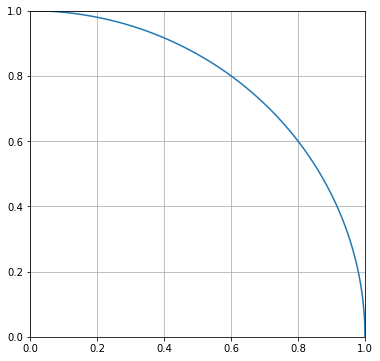
\includegraphics[keepaspectratio,alt={png}]{../images/activity-mc_integration_activity-mc_integration_tmp_3_0.png}}
\caption{png}
\end{figure}

\subsubsection{The Drop Algorithm}\label{the-drop-algorithm}

The concept behind this is watching rain hit the ground and counting the
droplets inside and outside a circle. We can simulate this with random
drops in the range from 0 to 1 in \(x\) and \(y\). Let's start with 500
drops. We plot the drops below.

\begin{Shaded}
\begin{Highlighting}[]
\NormalTok{ndrops }\OperatorTok{=} \DecValTok{500}
\NormalTok{drops }\OperatorTok{=}\NormalTok{ np.zeros([ndrops,}\DecValTok{2}\NormalTok{])}

\ControlFlowTok{for}\NormalTok{ i }\KeywordTok{in} \BuiltInTok{range}\NormalTok{(ndrops):}
    
\NormalTok{    xrand }\OperatorTok{=}\NormalTok{ random.random()}
\NormalTok{    yrand }\OperatorTok{=}\NormalTok{ random.random()}
    
\NormalTok{    drops[i] }\OperatorTok{=}\NormalTok{ xrand,yrand}
\end{Highlighting}
\end{Shaded}

\begin{Shaded}
\begin{Highlighting}[]
\NormalTok{plt.figure(figsize}\OperatorTok{=}\NormalTok{(}\DecValTok{6}\NormalTok{,}\DecValTok{6}\NormalTok{))}

\NormalTok{plt.plot(x,y)}

\NormalTok{plt.scatter(drops[:,}\DecValTok{0}\NormalTok{],drops[:,}\DecValTok{1}\NormalTok{], c}\OperatorTok{=}\StringTok{\textquotesingle{}C1\textquotesingle{}}\NormalTok{)}

\NormalTok{plt.axis([}\DecValTok{0}\NormalTok{, }\DecValTok{1}\NormalTok{, }\DecValTok{0}\NormalTok{, }\DecValTok{1}\NormalTok{])}
\NormalTok{plt.grid()}
\end{Highlighting}
\end{Shaded}

\begin{figure}
\centering
\pandocbounded{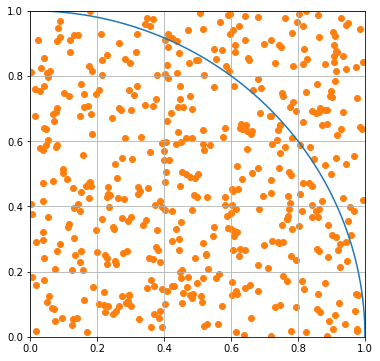
\includegraphics[keepaspectratio,alt={png}]{../images/activity-mc_integration_activity-mc_integration_tmp_6_0.png}}
\caption{png}
\end{figure}

Notice that some of the drops are outside the curve and some are inside.
We can use the formula for a circle of radius 1 to find which are which.

\[x^2 + y^2 = 1\]

If this produce is below 1, the drop is inside the curve; otherwise it's
outside. The statement below forms a binary filter. You might have seen
something like this before in CMSE 201. We can use those filters on the
arrays are replot to confirm. The use of of the tilde (\textasciitilde)
reverses the filter (true becomes false and vice versa).

\begin{Shaded}
\begin{Highlighting}[]
\NormalTok{insideCurve }\OperatorTok{=}\NormalTok{ drops[:,}\DecValTok{0}\NormalTok{]}\OperatorTok{**}\DecValTok{2}\OperatorTok{+}\NormalTok{drops[:,}\DecValTok{1}\NormalTok{]}\OperatorTok{**}\DecValTok{2} \OperatorTok{\textless{}} \DecValTok{1}

\NormalTok{plt.figure(figsize}\OperatorTok{=}\NormalTok{(}\DecValTok{8}\NormalTok{,}\DecValTok{8}\NormalTok{))}

\NormalTok{plt.plot(x, y, label}\OperatorTok{=}\StringTok{\textquotesingle{}circle\textquotesingle{}}\NormalTok{)}

\NormalTok{plt.scatter(drops[insideCurve,}\DecValTok{0}\NormalTok{],drops[insideCurve,}\DecValTok{1}\NormalTok{], c}\OperatorTok{=}\StringTok{\textquotesingle{}C1\textquotesingle{}}\NormalTok{, label}\OperatorTok{=}\StringTok{\textquotesingle{}inside\textquotesingle{}}\NormalTok{)}
\NormalTok{plt.scatter(drops[}\OperatorTok{\textasciitilde{}}\NormalTok{insideCurve,}\DecValTok{0}\NormalTok{],drops[}\OperatorTok{\textasciitilde{}}\NormalTok{insideCurve,}\DecValTok{1}\NormalTok{], c}\OperatorTok{=}\StringTok{\textquotesingle{}C2\textquotesingle{}}\NormalTok{, label}\OperatorTok{=}\StringTok{\textquotesingle{}outside\textquotesingle{}}\NormalTok{)}

\NormalTok{plt.axis([}\DecValTok{0}\NormalTok{, }\DecValTok{1}\NormalTok{, }\DecValTok{0}\NormalTok{, }\DecValTok{1}\NormalTok{])}
\NormalTok{plt.grid()}
\end{Highlighting}
\end{Shaded}

\begin{figure}
\centering
\pandocbounded{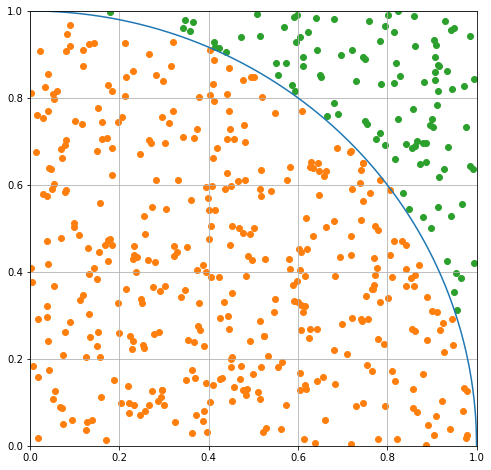
\includegraphics[keepaspectratio,alt={png}]{../images/activity-mc_integration_activity-mc_integration_tmp_8_0.png}}
\caption{png}
\end{figure}

\subsubsection{Computing Pi}\label{computing-pi}

We assumed our approach would bear out a constant.

\[c=\dfrac{A_{circle}}{A_{square}}\]

We can compute an estimate of it using the number of drops, which are
proxies for the area of a quarter circle.

\[c \approx 4\dfrac{N_{inside}}{N}\]

Our estimate is below.

\begin{Shaded}
\begin{Highlighting}[]
\NormalTok{pi\_estimate }\OperatorTok{=} \DecValTok{4}\OperatorTok{*}\BuiltInTok{len}\NormalTok{(drops[insideCurve])}\OperatorTok{/}\BuiltInTok{len}\NormalTok{(drops)}
\BuiltInTok{print}\NormalTok{(pi\_estimate)}
\end{Highlighting}
\end{Shaded}

\begin{verbatim}
3.152
\end{verbatim}

\subsection{Seeking Convergence}\label{seeking-convergence}

So the estimate was probably not great. But we can make it better by
choosing more drops. So rewrite this approach a function where you can
send the number of drops in and return the estimate of pi. Then use it
to plot this estimate over many choices of N. Show what the value
converges to.

\begin{Shaded}
\begin{Highlighting}[]
\CommentTok{\#\# your code here}
\end{Highlighting}
\end{Shaded}

\subsection{Finding the values of
integrals}\label{finding-the-values-of-integrals}

So that was a cool trick, but the power of this form of Monte Carlo is
being able to compute very difficult integrals. It's not efficient as
other integrators, but it's sometimes the only choice.

\subsubsection{Integrating sine}\label{integrating-sine}

Using the same approach as before where we take the proportion of drops
`under the curve' compared to all drops, find the integral of \(sin(x)\)
over one interval.

\begin{itemize}
\tightlist
\item
  Find the number of drops needed to make a reasonable estimate.
\item
  Use the long term behavior (plot it?) to estimate the value and
  uncertainty in the integral
\end{itemize}

\begin{Shaded}
\begin{Highlighting}[]
\CommentTok{\#\# your code here}
\end{Highlighting}
\end{Shaded}

\subsubsection{A Pathologically Terrible
Integral}\label{a-pathologically-terrible-integral}

Consider the function below over the interval from 0 to 2.

\[y = \sin^2\left[\dfrac{1}{x(2-x)}\right]\]

Let's plot this son of gun.

\begin{Shaded}
\begin{Highlighting}[]
\NormalTok{x }\OperatorTok{=}\NormalTok{ np.arange(}\FloatTok{0.00001}\NormalTok{,}\DecValTok{2}\NormalTok{,}\FloatTok{0.00001}\NormalTok{)}
\NormalTok{y }\OperatorTok{=}\NormalTok{ np.sin(}\DecValTok{1}\OperatorTok{/}\NormalTok{(x}\OperatorTok{*}\NormalTok{(}\DecValTok{2}\OperatorTok{{-}}\NormalTok{x)))}\OperatorTok{**}\DecValTok{2}

\NormalTok{plt.figure(figsize}\OperatorTok{=}\NormalTok{(}\DecValTok{8}\NormalTok{,}\DecValTok{8}\NormalTok{))}
\NormalTok{plt.plot(x,y)}
\NormalTok{plt.axis([}\DecValTok{0}\NormalTok{, }\DecValTok{2}\NormalTok{, }\DecValTok{0}\NormalTok{, }\DecValTok{1}\NormalTok{])}
\NormalTok{plt.grid()}
\end{Highlighting}
\end{Shaded}

\begin{figure}
\centering
\pandocbounded{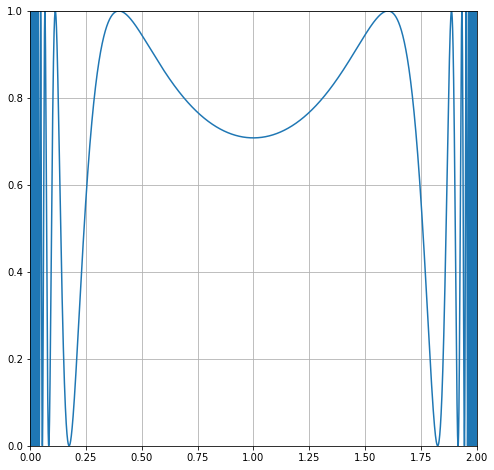
\includegraphics[keepaspectratio,alt={png}]{../images/activity-mc_integration_activity-mc_integration_tmp_16_0.png}}
\caption{png}
\end{figure}

Let's zoom in on one of the wings, and we can see the problem. The
integral varies wildly!

\begin{Shaded}
\begin{Highlighting}[]
\NormalTok{x }\OperatorTok{=}\NormalTok{ np.arange(}\FloatTok{0.00001}\NormalTok{,}\DecValTok{2}\NormalTok{,}\FloatTok{0.00001}\NormalTok{)}
\NormalTok{y }\OperatorTok{=}\NormalTok{ np.sin(}\DecValTok{1}\OperatorTok{/}\NormalTok{(x}\OperatorTok{*}\NormalTok{(}\DecValTok{2}\OperatorTok{{-}}\NormalTok{x)))}\OperatorTok{**}\DecValTok{2}

\NormalTok{plt.figure(figsize}\OperatorTok{=}\NormalTok{(}\DecValTok{8}\NormalTok{,}\DecValTok{8}\NormalTok{))}
\NormalTok{plt.plot(x,y)}
\NormalTok{plt.axis([}\FloatTok{1.75}\NormalTok{, }\DecValTok{2}\NormalTok{, }\DecValTok{0}\NormalTok{, }\DecValTok{1}\NormalTok{])}
\NormalTok{plt.grid()}
\end{Highlighting}
\end{Shaded}

\begin{figure}
\centering
\pandocbounded{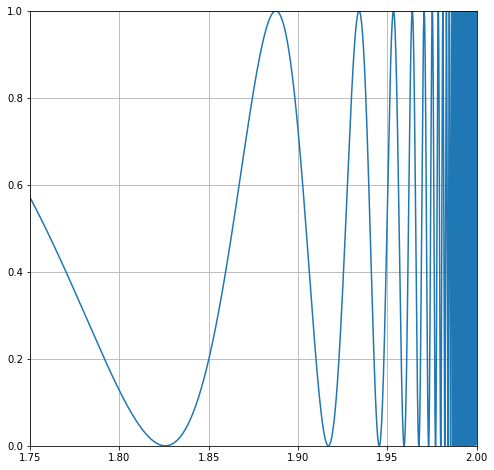
\includegraphics[keepaspectratio,alt={png}]{../images/activity-mc_integration_activity-mc_integration_tmp_18_0.png}}
\caption{png}
\end{figure}

\subsection{Bring in Monte Carlo}\label{bring-in-monte-carlo}

Following the same approach estimate the value of the integral for this
function and the uncertainty in your estimate.

\begin{Shaded}
\begin{Highlighting}[]
\CommentTok{\#\# your code here}
\end{Highlighting}
\end{Shaded}
